\documentclass{beamer}

\usetheme{Madrid}      % 内置主题(推荐新手使用)
\useoutertheme{miniframes} % 外层主题:横向小方块目录条
% \usetheme{Frankfurt}
% \usepackage[x11names]{xcolor}  % 加载扩展色库
% \usecolortheme[named=OliveDrab3]{structure}  % 柔和绿色

\title{Wavelet Transform for Image Processing}
\author{
\texorpdfstring{
Zhang Jinrui\thanks{alternative email:zhangjr1022@mails.jlu.edu.cn}
\\
He Jiashun
\\
Meng Jingyuan
\\
Jiang Zishen
\\
Mo Zian
}
{
Zhang Jinrui\thanks{alternative email:zhangjr1022@mails.jlu.edu.cn}
,
He Jiashun
,
Meng Jingyuan
,
Jiang Zishen
,
Mo Zian
}
}
\date{\today}

\begin{document}

\frame{\titlepage}  % 首页封面

\section{Pre-Processing}
% Slide 1: Background and Motivation
\begin{frame}{Background and Motivation}
    \begin{itemize}
        \item Image preprocessing is a crucial step in modern computer vision and machine learning.
        \item Models often require input images to have a fixed size and consistent format.
        \item Our goal is to convert any input image into a standardized grayscale format of size $2^N \times 2^N$.
        \item This not only simplifies downstream processing but also ensures compatibility with wavelet transform techniques, which rely on consistent input dimensions.
    \end{itemize}
\end{frame}

% Slide 2: Wavelet Transform Overview
\begin{frame}{Wavelet Transform Overview}
    \begin{itemize}
        \item The wavelet transform is a powerful mathematical tool for analyzing signals at multiple scales.
        \item Unlike the Fourier transform, which only reveals frequency content, wavelets provide both frequency and spatial localization.
        \item This is particularly useful in image processing where textures, edges, and fine structures need to be captured at different resolutions.
        \item Common wavelet families include Haar, Daubechies, and Coiflets — all benefit from inputs with dimensions that are powers of two.
    \end{itemize}
\end{frame}

% Slide 3: Image Processing Workflow
\begin{frame}{Image Processing Workflow}
    \begin{enumerate}
        \item \textbf{Image Loading and Grayscale Conversion}: The image is loaded using a Python imaging library and converted to grayscale. This reduces data complexity and focuses analysis on structural content.
        \item \textbf{Rescaling with Aspect Ratio Preservation}: The image is resized using high-fidelity interpolation to ensure one side reaches the target length ($2^N$), without distortion.
        \item \textbf{Centered Cropping}: The resized image is cropped to $2^N \times 2^N$, ensuring input uniformity without compromising important visual features.
        \item \textbf{Matrix Output}: The final image is converted into a matrix format suitable for mathematical operations, storage, and machine learning integration.
    \end{enumerate}
\end{frame}

% Slide 4: Theoretical Justification
\begin{frame}{Theoretical Justification}
    \begin{itemize}
        \item Many wavelet algorithms are optimized for inputs whose dimensions are powers of two — enabling efficient recursive decomposition.
        \item Improper dimensions can introduce edge effects or truncation artifacts, degrading transform results.
        \item LANCZOS interpolation is used due to its ability to preserve edges and textures during resizing, which is critical for wavelet-based analysis.
        \item Converting to a 2D matrix makes the image directly usable for NumPy operations and compatible with machine learning frameworks like TensorFlow and PyTorch.
    \end{itemize}
\end{frame}

% Slide 5: Application Scenarios
\begin{frame}{Application Scenarios}
    \begin{itemize}
        \item \textbf{Educational Tools}: Demonstrate how images are converted, processed, and decomposed in the frequency domain.
        \item \textbf{Scientific Research}: Used in experiments where consistent image input is necessary, such as style transfer or anomaly detection.
        \item \textbf{Data Preprocessing}: Helps in preparing inputs for neural networks, especially for tasks that benefit from texture analysis like medical imaging or remote sensing.
        \item \textbf{Feature Engineering}: Enables extraction of localized frequency features for traditional machine learning models.
    \end{itemize}
\end{frame}

% Slide 6: Extension Opportunities
\begin{frame}{Extension Opportunities}
    \begin{itemize}
        \item \textbf{Multi-channel Support}: Extend to RGB or multi-spectral image processing for richer feature representations.
        \item \textbf{Batch Automation}: Apply the transformation to entire datasets, allowing integration into large-scale pipelines.
        \item \textbf{Visualization Tools}: Incorporate graphical interfaces to preview the original vs. transformed image and to display wavelet decomposition layers.
        \item \textbf{Parameter Tuning}: Allow users to experiment with different interpolation methods or wavelet bases interactively.
    \end{itemize}
\end{frame}

% Slide 7: Conclusion
\begin{frame}{Conclusion}
    \begin{itemize}
        \item The image conversion program serves as a foundational tool that bridges raw image data and advanced analysis techniques.
        \item Its adherence to standardized formats makes it ideal for educational purposes, algorithm development, and production pipelines.
        \item Future development can make it even more powerful by supporting color analysis, batch operations, and intuitive visual feedback.
    \end{itemize}
\end{frame}

\section{Haar Compression}
\begin{frame}
    \frametitle{Standard Haar Decomposition}
    \begin{itemize}
        \item sdlfkj
        \item sDF
        \item sdf
    \end{itemize}
\end{frame}
\begin{frame}
    \frametitle{sfdfg}
    \begin{itemize}
        \item sdlfkj
        \item sDF
        \item sdf
    \end{itemize}
\end{frame}
\begin{frame}
    \frametitle{sadsgkjh}
    \begin{itemize}
        \item sdlfkj
        \item sDF
        \item sdf
    \end{itemize}
\end{frame}
\begin{frame}
    \frametitle{sdf}
    \begin{itemize}
        \item sdlfkj
        \item sDF
        \item sdf
    \end{itemize}
\end{frame}

\section{Haar Compression Augmented}
\begin{frame}
    \frametitle{Basic Idea}
    \begin{itemize}
        \item \[
                  \sum_{k=1}^{n}\hat{l}_k^4
                  \leq
                  (\sum_{k=1}^{n}\hat{l}_k^2)^2
                  =
                  (\sum_{k=1}^{n}l_k^2)^2
              \]
        \item \[
                  \min_{\hat{l}_k\in l^2 st. \sum_{k=1}^{n}\hat{l}_k^2=\sum_{k=1}^{n}l_k^2}(-\sum_{k=1}^{n}\hat{l}_k^4)
              \]
    \end{itemize}
\end{frame}
\begin{frame}
    \frametitle{Basic Idea}
    \begin{itemize}
        \item 	\begin{figure}
                  \centering
                  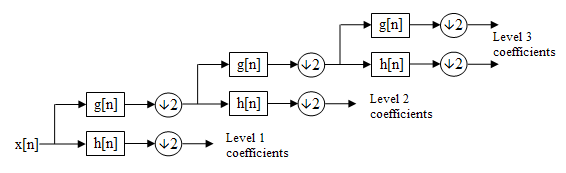
\includegraphics[width=0.8\textwidth]{fig/Wavelets_-_Filter_Bank.png}
                  \caption{Cascading}
                  \label{fig:Cascading}
              \end{figure}
        \item \[
                  \min_{\Phi}(-\sum_{k=1}^{n}\hat{l}_k^4)
              \]
        \item Condense the energy to as less coefficients as possible.
    \end{itemize}
\end{frame}
\begin{frame}
    \frametitle{Results}
    \begin{itemize}
        \item
              \begin{figure}[ht!]
                  \centering
                  \begin{minipage}{0.45\textwidth}
                      \centering
                      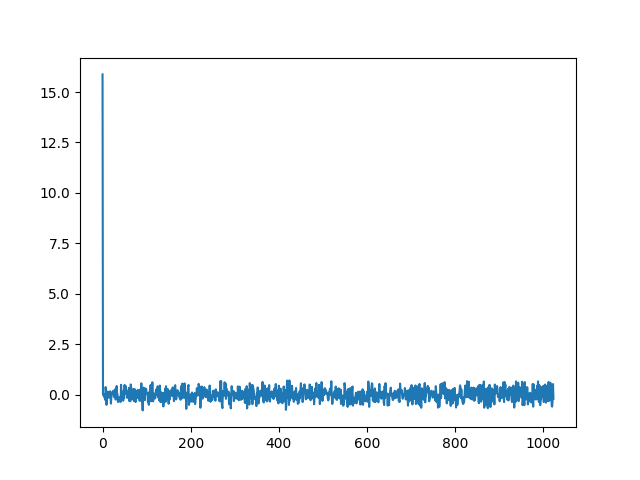
\includegraphics[width=0.9\textwidth]{fig/HaarAugmented1D_freq.png} % first figure itself
                      \caption{Haar 2x2 filter bank random input. Compression Rate 0.2568}
                      \label{fig:Haar}
                  \end{minipage}\hfill
                  \begin{minipage}{0.45\textwidth}
                      \centering
                      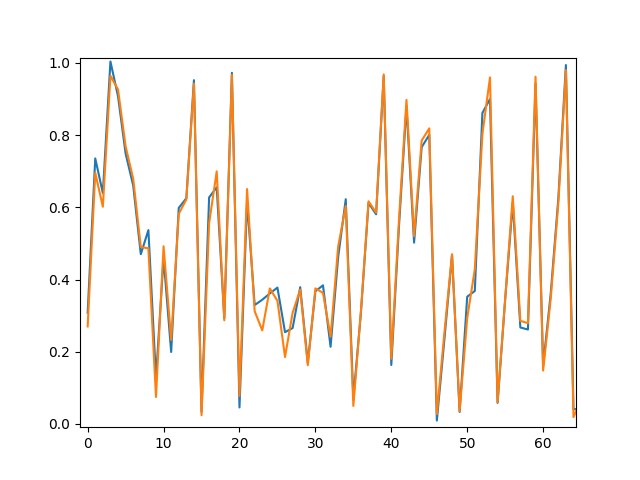
\includegraphics[width=0.9\textwidth]{fig/HaarAugmented1D_rec.png} % second figure itself
                      \caption{Haar 2x2 filter bank random input.Total average energy loss 0.0009}
                  \end{minipage}
              \end{figure}
              %   \begin{figure}
              %       \centering
              %       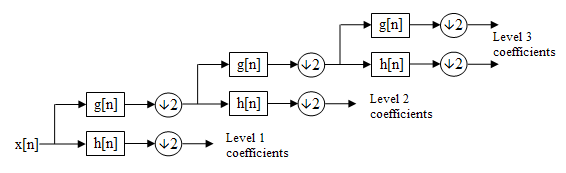
\includegraphics[width=0.8\textwidth]{fig/Wavelets_-_Filter_Bank.png}
              %       \caption{Siakam won 2025 NBA eastern conference finals MVP}
              %       \label{fig:Siakam}
              %   \end{figure}
        \item random sequence would take more information entropy so have a low compress rate.
    \end{itemize}
\end{frame}
\begin{frame}
    \frametitle{Results}
    \begin{itemize}
        \item
              \begin{figure}[ht!]
                  \centering
                  \begin{minipage}{0.45\textwidth}
                      \centering
                      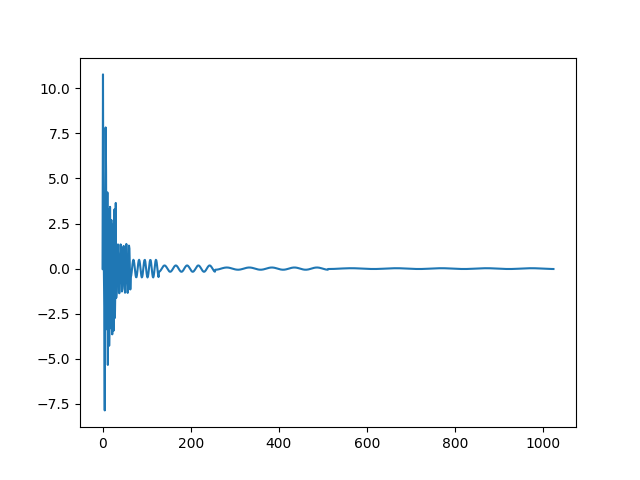
\includegraphics[width=0.9\textwidth]{fig/HaarAugmented1D_sin_freq.png} % first figure itself
                      \caption{Haar 2x2 filter bank sin input frequency. Compression Rate 0.9287}
                      \label{fig:Haar_sin}
                  \end{minipage}\hfill
                  \begin{minipage}{0.45\textwidth}
                      \centering
                      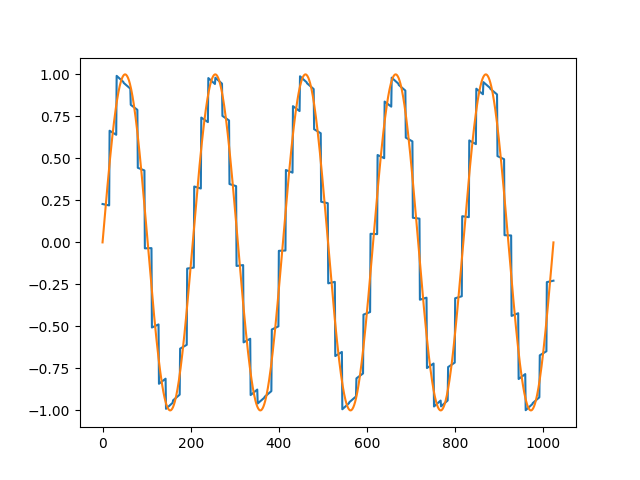
\includegraphics[width=0.9\textwidth]{fig/HaarAugmented1D_sin_rec.png} % second figure itself
                      \caption{Haar 2x2 filter bank sin input reconstruction.Total average energy loss 0.0104}
                  \end{minipage}
              \end{figure}
              %   \begin{figure}
              %       \centering
              %       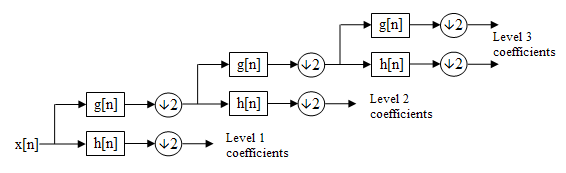
\includegraphics[width=0.8\textwidth]{fig/Wavelets_-_Filter_Bank.png}
              %       \caption{Siakam won 2025 NBA eastern conference finals MVP}
              %       \label{fig:Siakam}
              %   \end{figure}
        \item a smooth signal not have much information entropy, so will have a high compress rate.
    \end{itemize}
\end{frame}
\begin{frame}
    \frametitle{Results}
    \begin{itemize}
        \item
              \begin{figure}[ht!]
                  \centering
                  \begin{minipage}{0.45\textwidth}
                      \centering
                      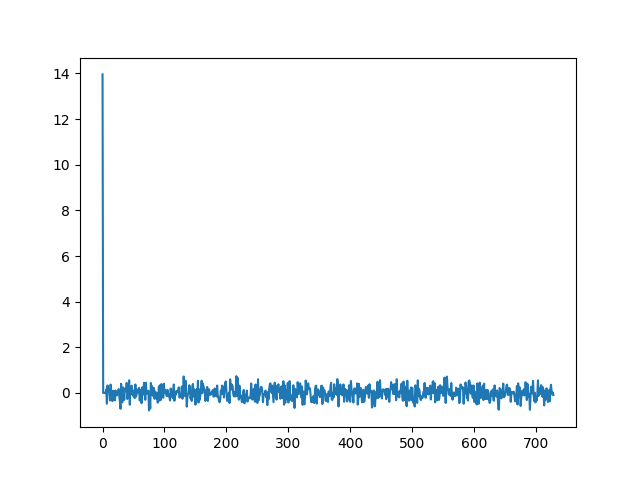
\includegraphics[width=0.9\textwidth]{fig/Haar3Augmented1D_freq.png} % first figure itself
                      \caption{Haar 3x3 filter bank random input. Compression Rate 0.1906}
                      \label{fig:Haar3}
                  \end{minipage}\hfill
                  \begin{minipage}{0.45\textwidth}
                      \centering
                      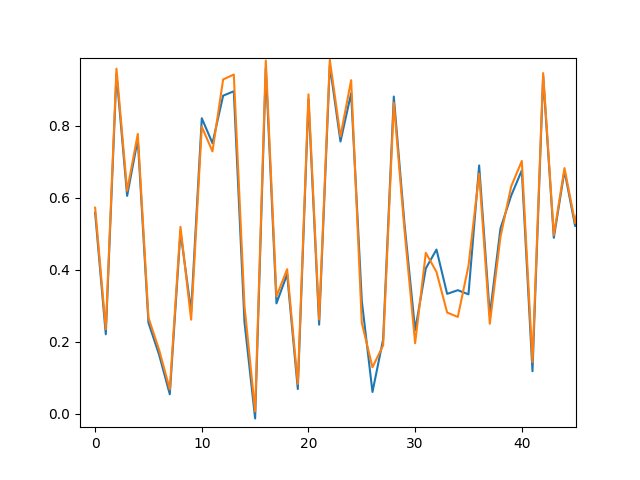
\includegraphics[width=0.9\textwidth]{fig/Haar3Augmented1D_rec.png} % second figure itself
                      \caption{Haar 3x3 filter bank random input.Total average energy loss 0.0008}
                  \end{minipage}
              \end{figure}
              %   \begin{figure}
              %       \centering
              %       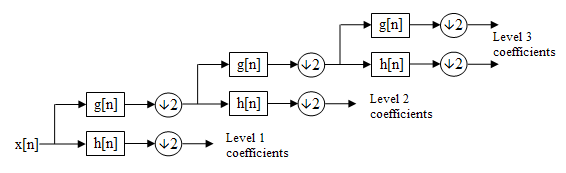
\includegraphics[width=0.8\textwidth]{fig/Wavelets_-_Filter_Bank.png}
              %       \caption{Siakam won 2025 NBA eastern conference finals MVP}
              %       \label{fig:Siakam}
              %   \end{figure}
        \item same random sequence same reason.
    \end{itemize}
\end{frame}
\begin{frame}
    \frametitle{Results}
    \begin{itemize}
        \item
              \begin{figure}[ht!]
                  \centering
                  \begin{minipage}{0.45\textwidth}
                      \centering
                      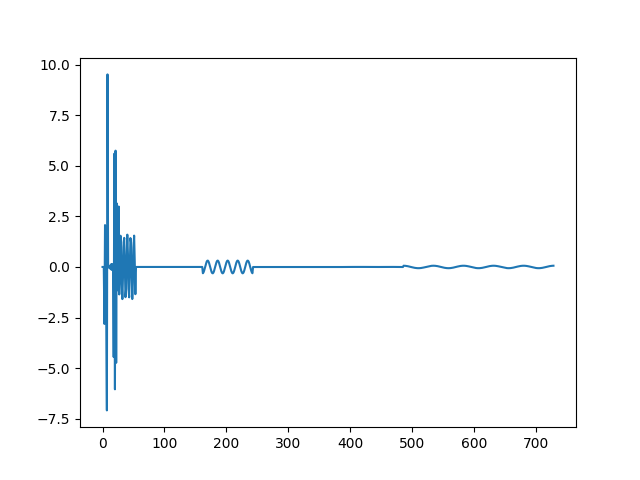
\includegraphics[width=0.9\textwidth]{fig/Haar3Augmented1D_sin_freq.png} % first figure itself
                      \caption{Haar 3x3 filter bank sin input frequency. Compression Rate 0.7750}
                      \label{fig:Haar3_sin}
                  \end{minipage}\hfill
                  \begin{minipage}{0.45\textwidth}
                      \centering
                      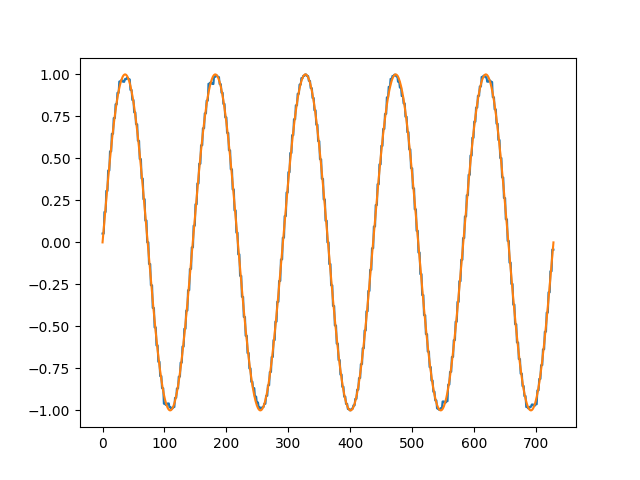
\includegraphics[width=0.9\textwidth]{fig/Haar3Augmented1D_sin_rec.png} % second figure itself
                      \caption{Haar 3x3 filter bank sin input reconstruction.Total average energy loss 0.0007}
                  \end{minipage}
              \end{figure}
              %   \begin{figure}
              %       \centering
              %       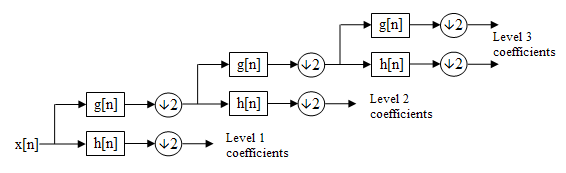
\includegraphics[width=0.8\textwidth]{fig/Wavelets_-_Filter_Bank.png}
              %       \caption{Siakam won 2025 NBA eastern conference finals MVP}
              %       \label{fig:Siakam}
              %   \end{figure}
        \item same smooth signal same reason.
    \end{itemize}
\end{frame}

\section{Zishen Jiang}
\begin{frame}
    \frametitle{sadsgkjh}
    \begin{itemize}
        \item sdlfkj
        \item sDF
        \item sdf
    \end{itemize}
\end{frame}

\section{Energy Analysis}
\begin{frame}
    \frametitle{sdf}
    \begin{itemize}
        \item sdlfkj
        \item sDF
        \item sdf
    \end{itemize}
\end{frame}

\end{document}
